\documentclass{extarticle}
\usepackage[utf8]{inputenc}
\usepackage[T1]{fontenc}
\usepackage{graphicx}
\usepackage{caption}
\usepackage{subcaption}
\usepackage{graphicx}
\usepackage{amsmath, amsthm, amssymb}
\usepackage[backend=biber,style=numeric,natbib=true]{biblatex}
\usepackage[margin=1.1in]{geometry}
\usepackage{setspace}
\usepackage{parskip}
\usepackage{multirow}
\usepackage{array}
\usepackage{indentfirst}
\usepackage{booktabs}
\usepackage[bottom]{footmisc}
\setlength{\footnotesep}{0.7cm}
\setlength{\parindent}{1cm}

\setstretch{1.15}

\addbibresource{references.bib}

\title{Modelling of real-life MIP problems}
\author{The Ikunbelievable Group\footnotemark[1]}
\date{}

\begin{document}

\maketitle

\renewcommand{\thefootnote}{\fnsymbol{footnote}}
\footnotetext[1]{%
  The Ikunbelievable Group consists of four people who contributed equally to this work:
  \begin{tabular}{@{}l}
    Xiaotian Ji (\texttt{Xiaotian.Ji20@student.xjtlu.edu.cn}), \\
    Qiuyi Chen (\texttt{Qiuyi.Chen2002@student.xjtlu.edu.cn}), \\
    Liyuan Jin (\texttt{Liyuan.Jin20@student.xjtlu.edu.cn}),   \\
    Qin Chi (\texttt{Chi.Qin20@student.xjtlu.edu.cn}).%
  \end{tabular}%
}
\renewcommand{\thefootnote}{\arabic{footnote}}

\section{Introduction}

Lily has recently been accepted into a school at the London School of Economics
and Political Science, majored in Operational Research and her boyfriend,
David, is set to begin his studies at Imperial College London. Eager to make
the most of their summer vacation in Europe before the start of the school
term, they decide to embark on a memorable 2-week trip, exploring famous
European cities.

David, a music fan, has a strong desire to visit Vienna, while Lily wishes to
visit the Van Gogh Museum in Amsterdam. With their interests in mind, they
eventually select nine different destinations: Vienna, Paris, Rome, Barcelona,
Berlin, Amsterdam, Copenhagen, Zurich, and Budapest. They prefer traveling by
train and plane, but due to Lily's past witness of a traumatic plane crash,
they will limit the number of times that they take a plane.

In order to plan their sightseeing itinerary, the challenge lies in organizing
their routes under the constraints of time and cost, while also ensuring that
they visit all of their desired destinations, taking into account the varying
train and plane ticket prices. However, they have no idea to start with, so
they turn to the Ikunbelievable Group for help.

\section{Problem description}

\subsection{Input and Objective}

\begin{enumerate}
  \item Cities: For their graduation trip, they have chosen 10 representative cities,
        including London, Vienna, Paris, Barcelona, Berlin, Amsterdam, Copenhagen
        (København), Zurich, and Budapest.
  \item Transportation Options: They will consider to take plane or train to travel
        between these cities.
  \item Time: We will consider the time required to travel between cities by plane and
        train.
  \item Price: Since ticket prices can vary from month to month, in early May, we
        calculated the average price of tickets from July 1 to July 14 and from August
        1 to August 14 in 2023.
  \item Customization: To account for individual preferences, we will input different
        weights for cost and time, allowing each traveler to prioritize factors that
        are most important to them when selecting the optimal travel itinerary.
\end{enumerate}

Their objective is to find the optimal travel route under the assumptions and
the constraints described below.

\subsection{Assumptions}

We make the following assumptions in our analysis:

\begin{enumerate}
  \item The travel time and cost between city A and city B are identical in both
        directions.
  \item Two modes of transportation, train and plane, are considered, despite the
        existence of alternative choices.
  \item The trip must start and end in specific city and in their case, they have
        chosen London as the starting and ending point because we need to put our
        luggage in the school in London then only take some necessary things for the
        trip.
  \item Taking into account that ticket prices may be affected by various factors, such
        as public health events, peak travel seasons, etc, we selected and averaged all
        ticket prices between July 1st and July 14th, from 8 AM to 8 PM, to determine
        the ticket price. Similarly, we applied the same process for the period between
        August 1st and August 14th to reduce the impact of outliers, making the results
        more stable and reliable.\
\end{enumerate}

\subsection{Constraints}

Our objective is to find the optimal transportation options for different
groups of people with different demands, allowing for efficient travel across
all cities. In order to achieve this goal, some constraints are as followed:

\begin{enumerate}
  \item Each city can only be visited once.
  \item Due to some special reasons, the times for taking plane or train will be
        limited. For example, some people wouldn't like to take plane or train, some
        people have some coupons that allow them to eat food for free on airplanes or
        trains or they are the members of some airlines or train companies, so they can
        get some extra luxury services. Therefore, we set the maximum times for taking
        plane and train.
\end{enumerate}

\subsection{Toy Example}

Now we demonstrate a simple example to show the consequence of implementing different traveling routes.

\subsubsection{Input and Objective}
\begin{itemize}
  \item Cities: For the trip in the summer vocation, traveling from Anhui province to
        Guangdong Province, choose 3 representative cities, including Guangzhou,
        Shenzhen, and Foshan.
  \item Transportation Options: Only consider to take plane or train to travel between
        these cities.
  \item Time: Only consider the time required to travel between cities by plane and
        train.
  \item Price: The fares we use was the real price booking in June 2022.
  \item Customization: Only consider the total cost, and don't care about the time.
\end{itemize}

\subsubsection{Assumptions}
\begin{itemize}
  \item The travel time and cost between city A and city B are identical in both directions.
  \item Because of the distance, take plane from Anhui Province to Guangdong Province, and travel around the three cities in Guangdong Province by high-speed train.
  \item The trip starts and ends in Hefei.
  \item Each city can only be visited once.
\end{itemize}

The ticket prices as well as the possible traveling routes are as follows. Green lines mean the airplane routes, while the blue lines are represented the train routes.
Following the pink one, the total cost we spend is ¥1200, which is the optimal plan. Compared with the best choice, if we carry out the orange route, the sum of all ticket prices is ¥1645, which will increase the expense for nearly ¥450.


\begin{figure}[!ht]
  \centering
  \begin{subfigure}{0.3\textwidth}
      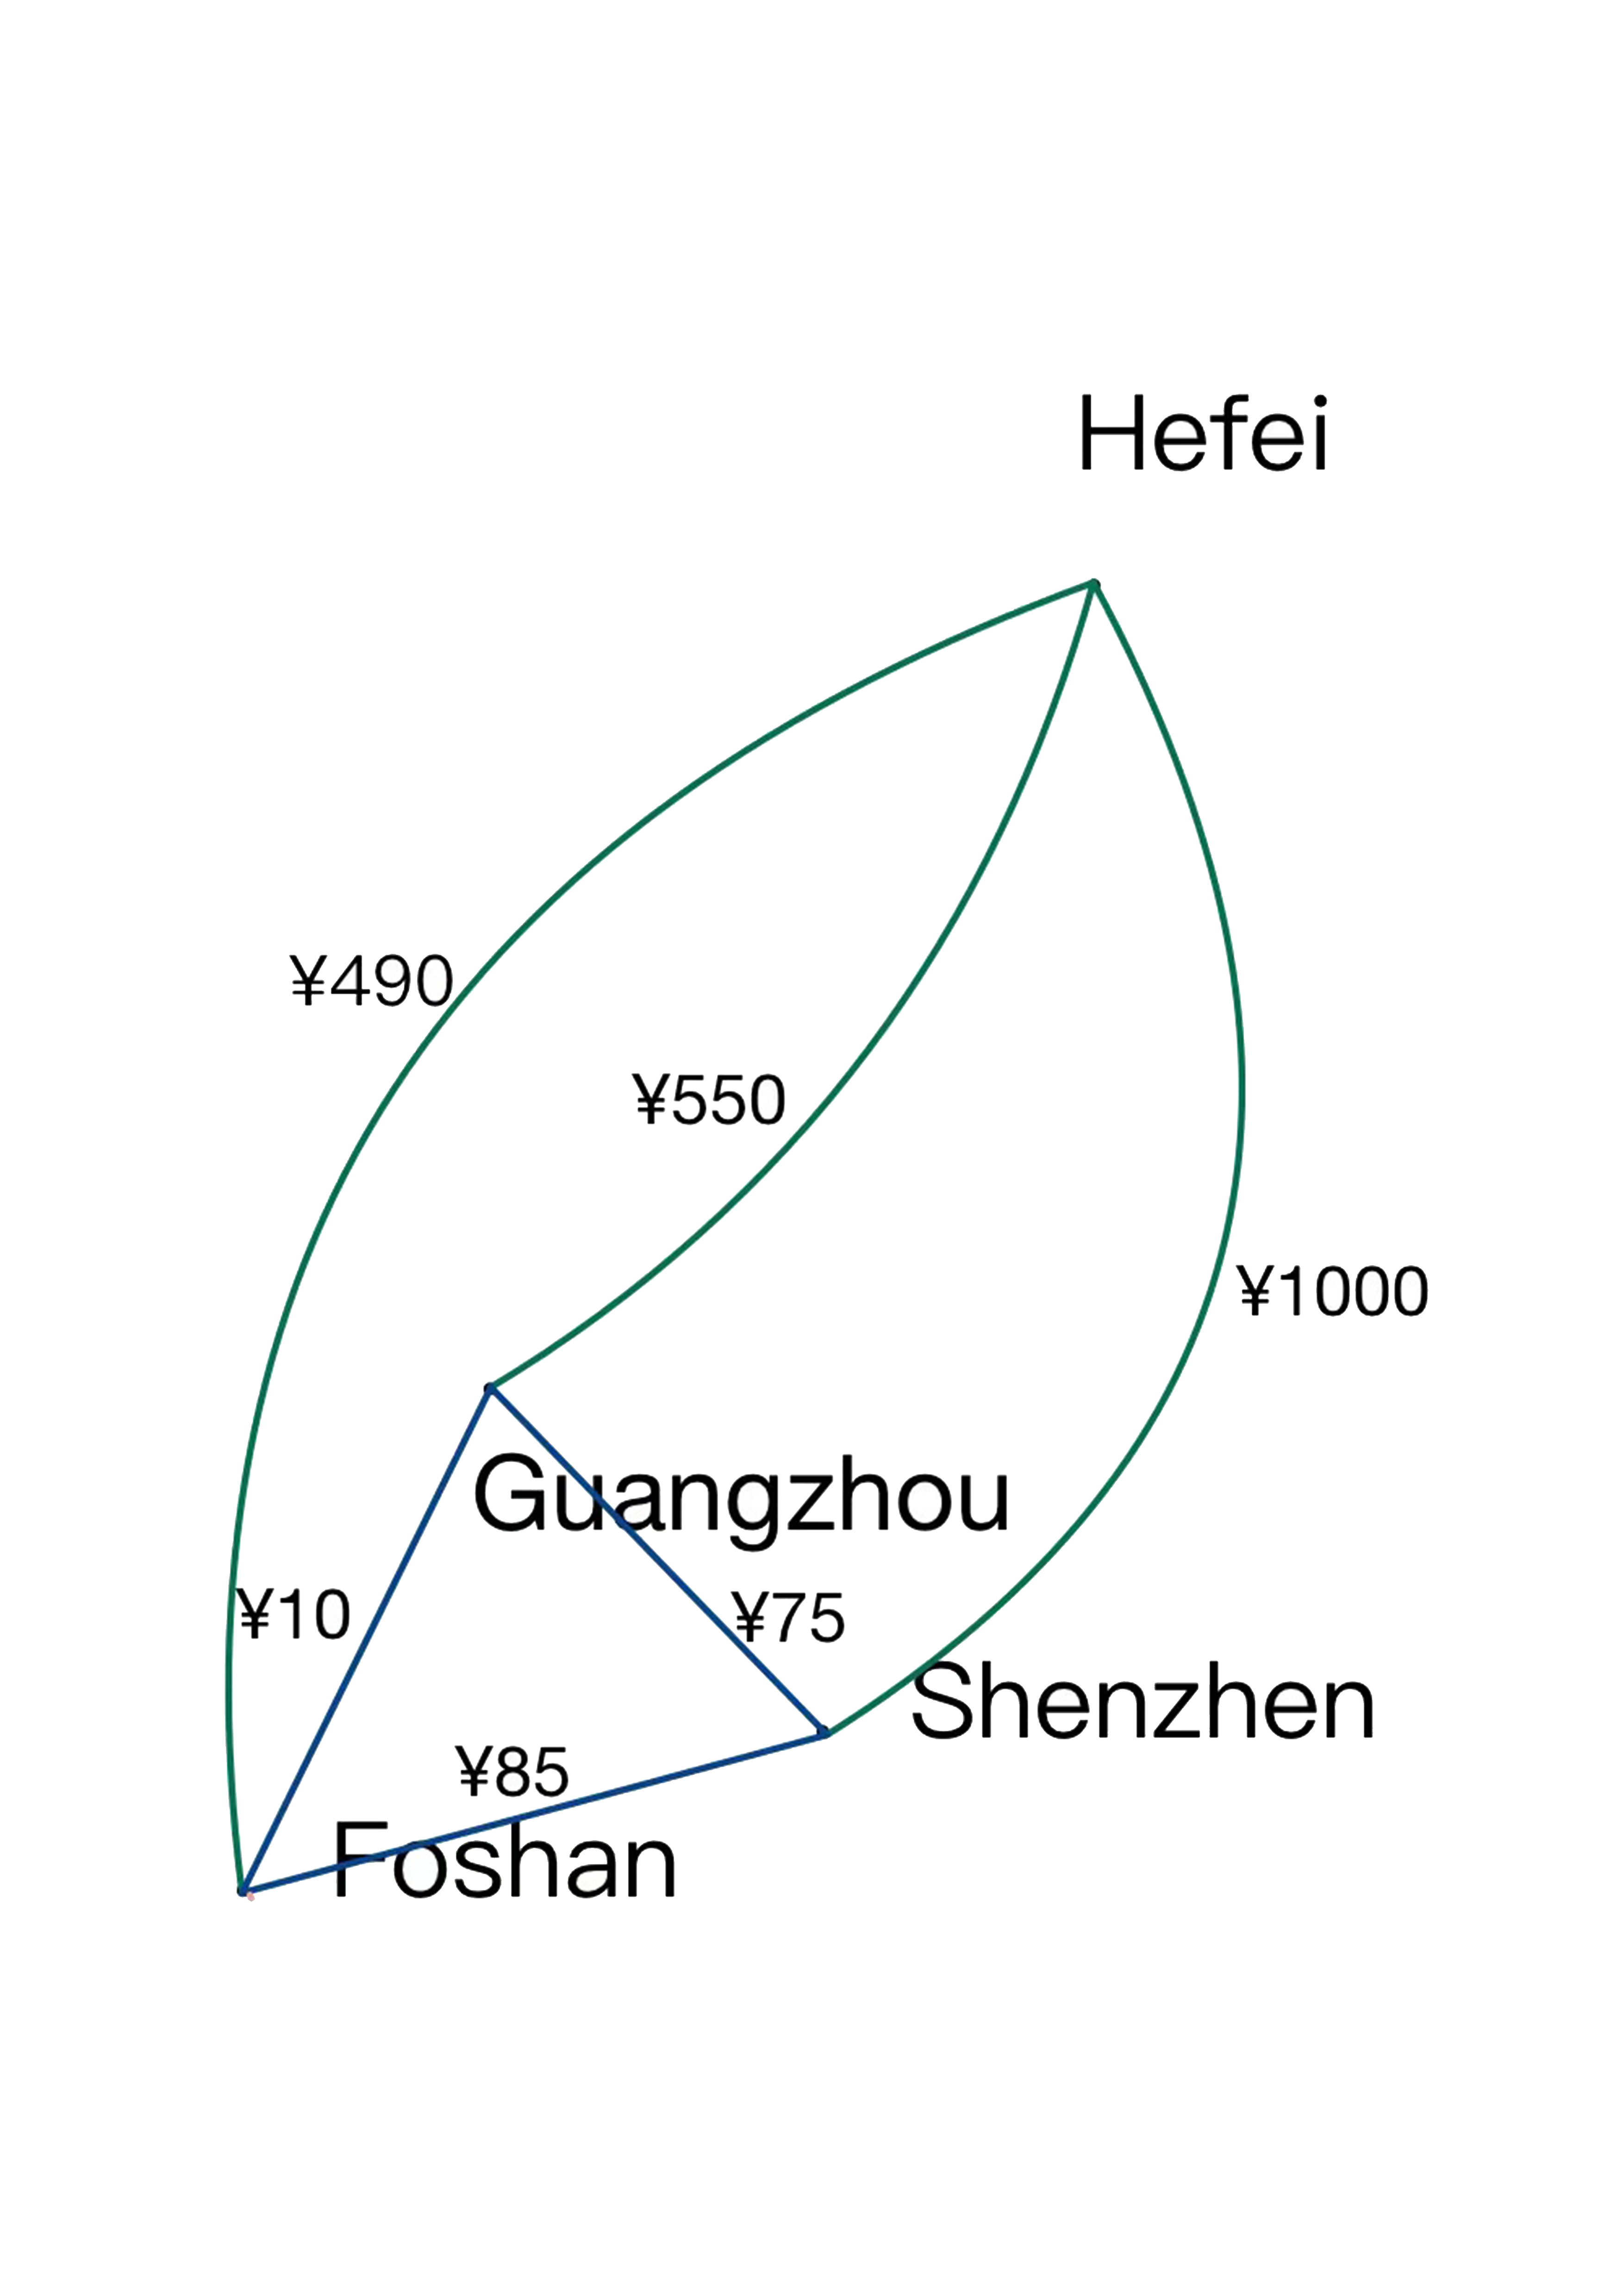
\includegraphics[width=\textwidth]{pic/1.png}
      \caption{Caption for your second image}%
\label{fig:your_image1}
  \end{subfigure}
  \hfill % Add space between images
  \begin{subfigure}{0.3\textwidth}
      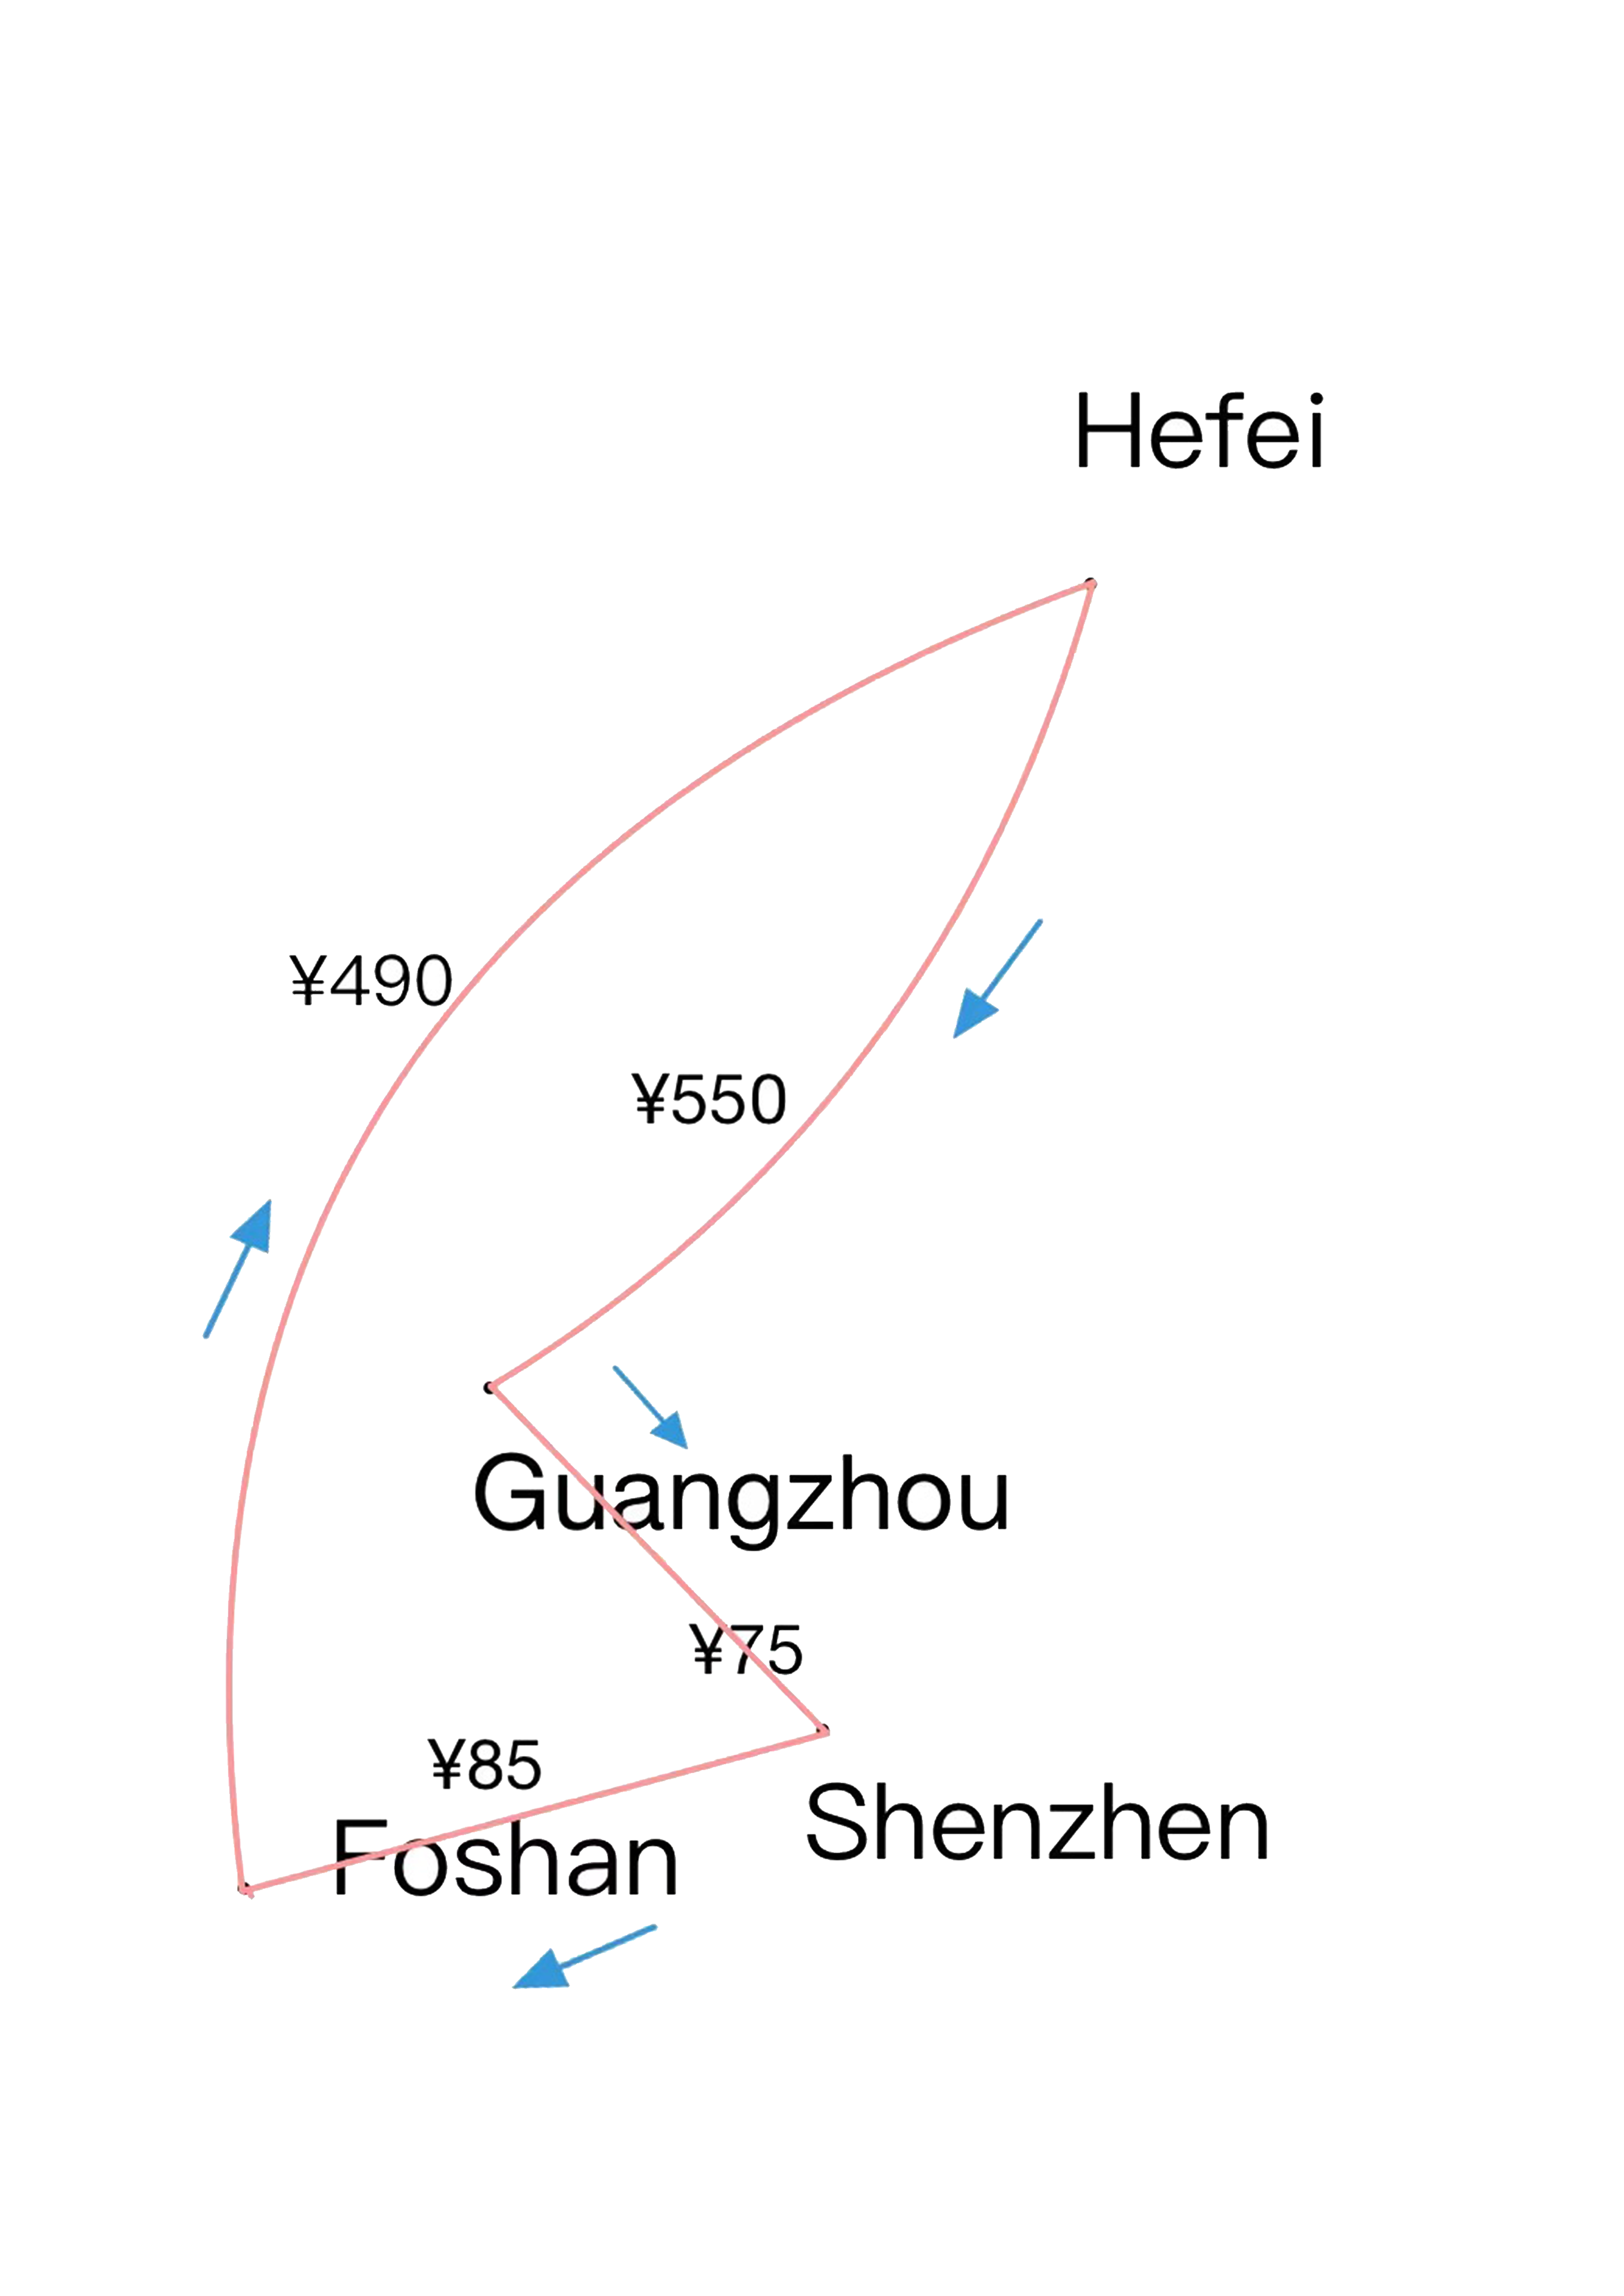
\includegraphics[width=\textwidth]{pic/2.png}
      \caption{Caption for your third image}%
\label{fig:your_image2}
  \end{subfigure}%
  \hfill % Add space between images
  \begin{subfigure}{0.3\textwidth}
      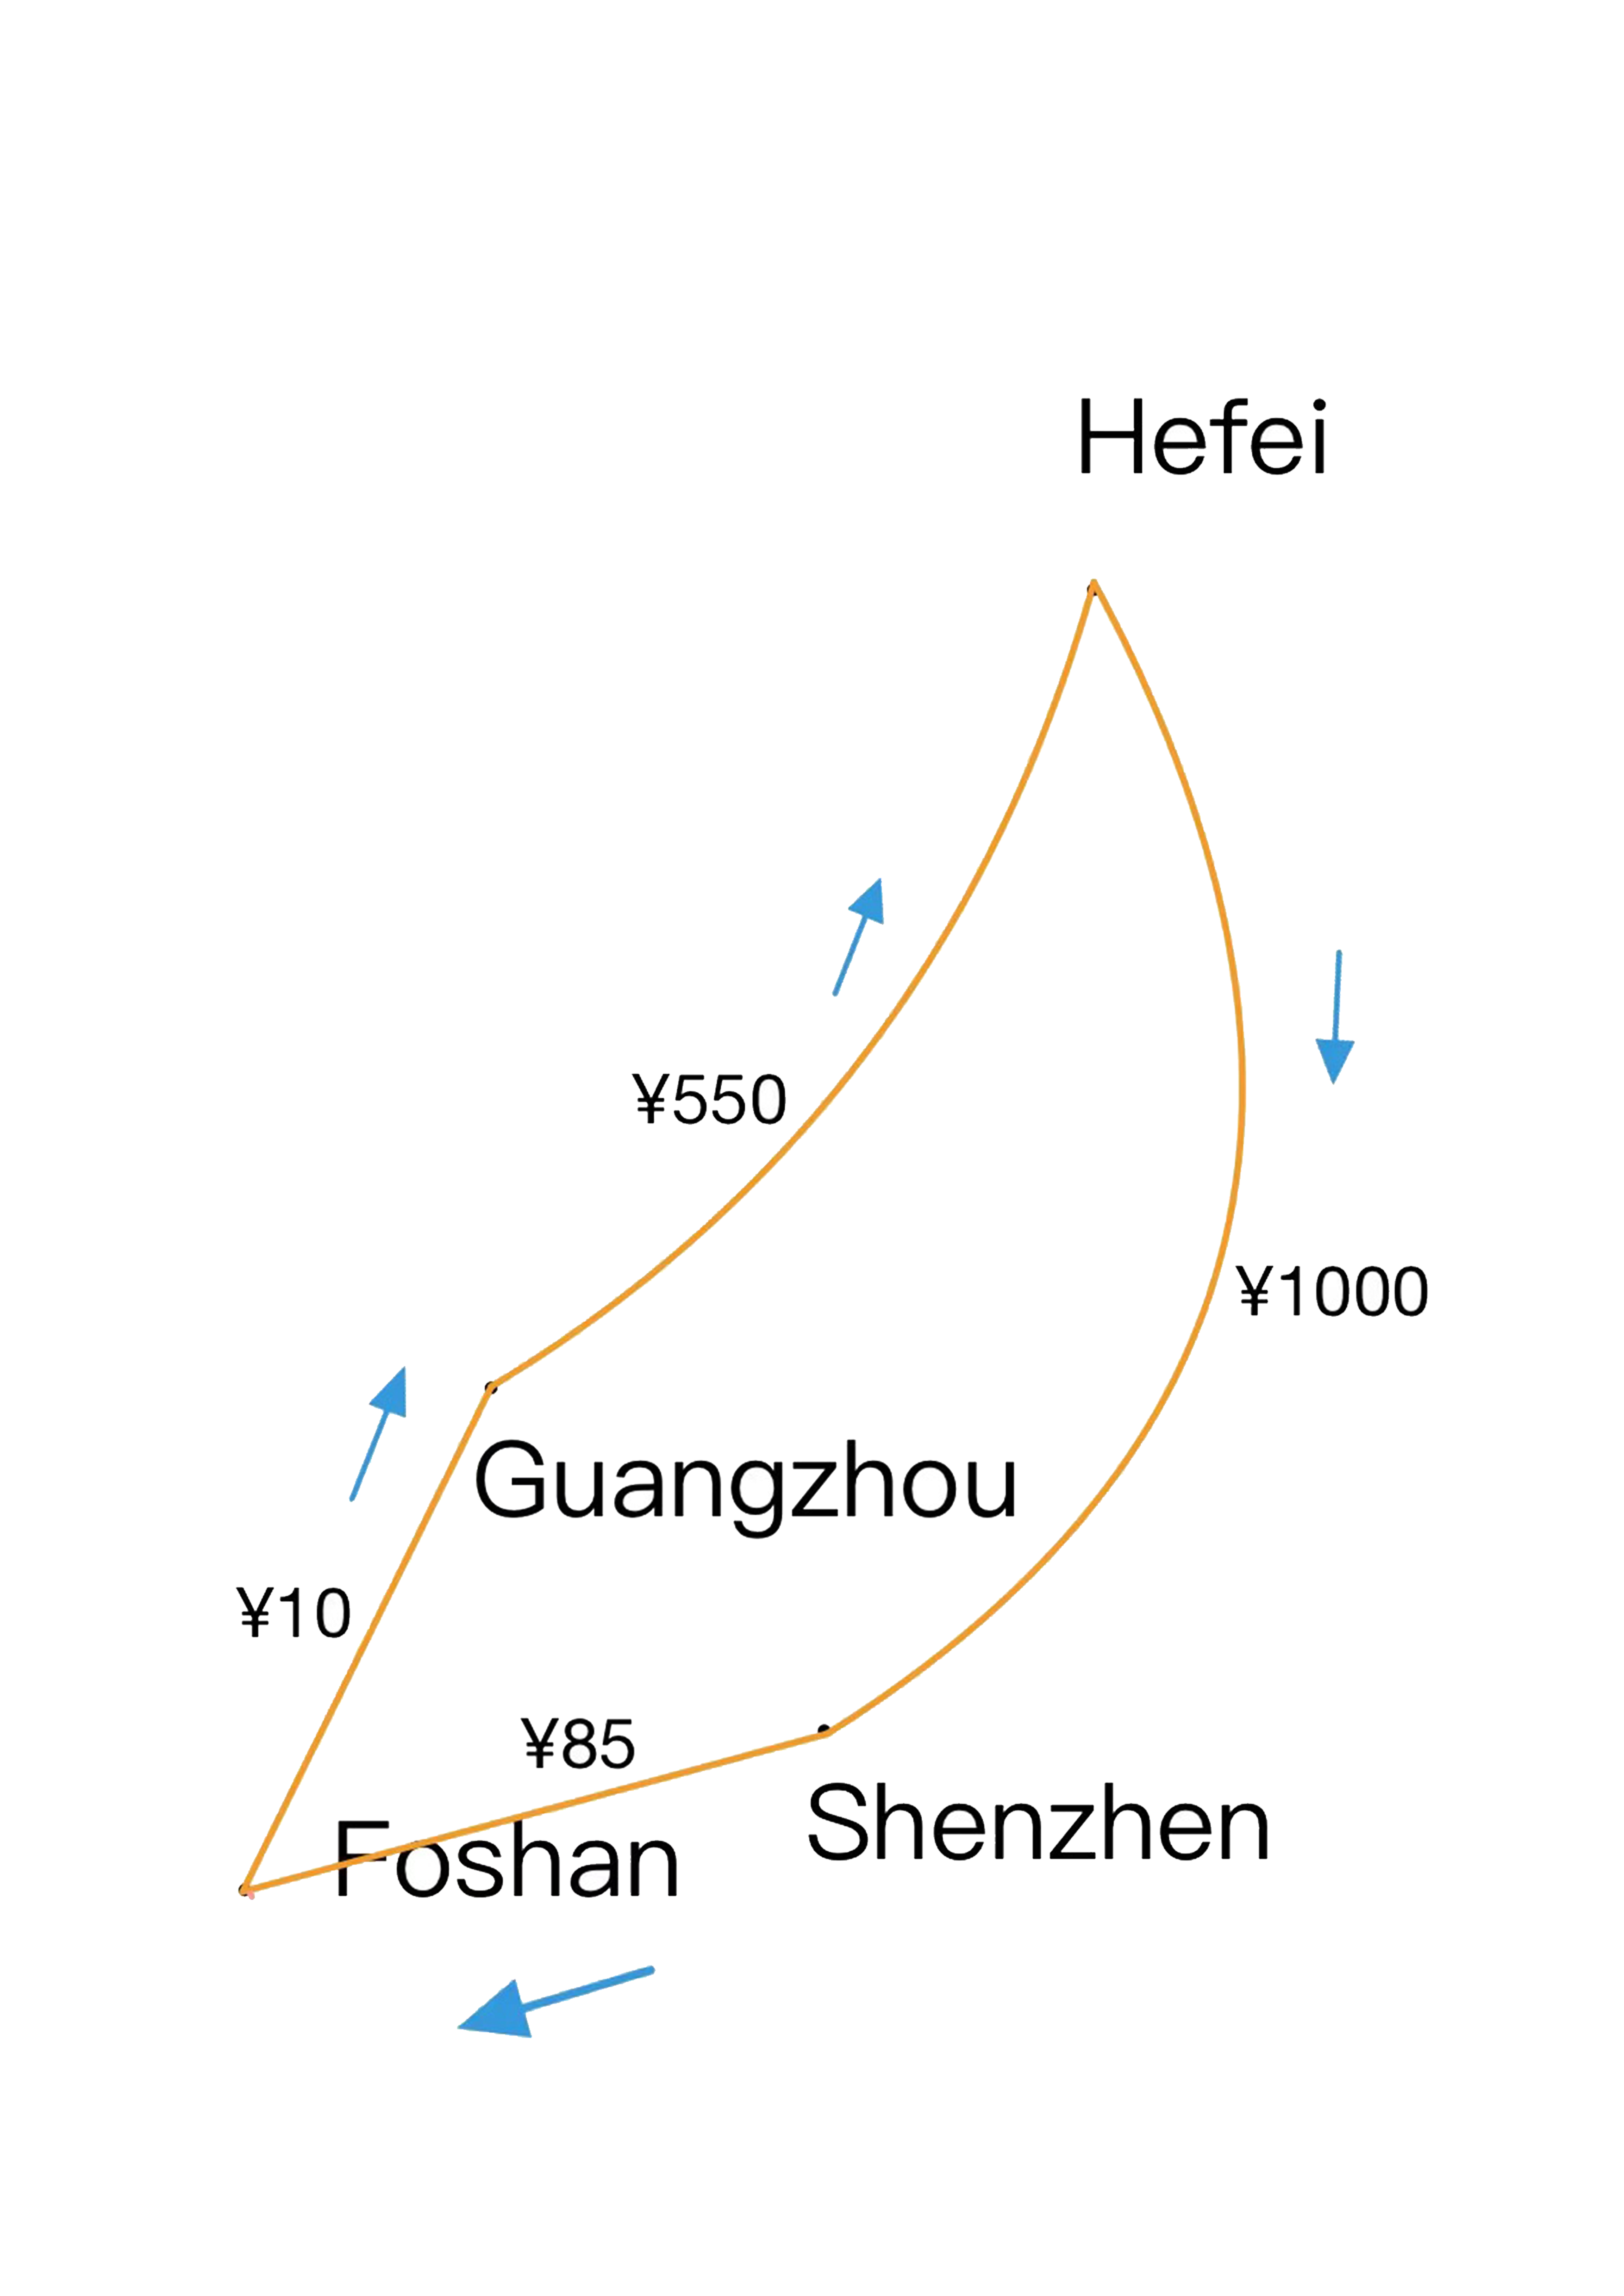
\includegraphics[width=\textwidth]{pic/3.png}
      \caption{Caption for your third image}%
\label{fig:your_image3}
  \end{subfigure}%
\end{figure}
\section{MIP Model}
Let $G_1(V_1, E_1)$ and $G_2(V_2, E_2)$ be two given graphs, each with their
respective vertex and edge sets. Define a positive edge weight function $w :
  E_1 \cup E_2 \rightarrow \mathbb{R}^+$. We construct a new graph $G(V, E)$,
where $V = V_1 \cup V_2$ and $E = E_1 \cup E_2$. The objective is to find a
Hamiltonian cycle in $G$ that minimizes the objective function. In order to
achieve this, we introduce binary variables $x_{ij}^k$ for edge selection from
either $G_1$ or $G_2$.

Formally, let $x_{ij}^k \in \{0, 1\}$ be a binary variable such that:

\begin{equation*}
  x_{ij}^k =
  \begin{cases}
    1, & \text{if edge } (i, j) \text{ from graph } G_k \text{ is selected,} \\
    0, & \text{otherwise.}
  \end{cases}
\end{equation*}

The goal is to determine the values of $x_{ij}^k$ that lead to a Hamiltonian
cycle with the minimum objective function value in the graph $G$. The objective
function to minimize can be written as:
\begin{equation*}
  \text{minimize} \, f = \sum_{k=1}^{2} \sum_{(i,j) \in E_k} w_{ij}^k x_{ij}^k
\end{equation*}

Subject to the following \textbf{constraints}:

\begin{enumerate}
  \item Each vertex has a total degree of 2, with one incoming edge (in-degree) and one
        outgoing edge (out-degree) from either graph $G_1$ or $G_2$.

        \begin{equation*}
          \sum_{k=1}^{2} \sum_{j \in V} x_{ij}^k = 2, \quad \forall i \in V
        \end{equation*}
  \item No subtours are allowed (subtour elimination constraint):

        \begin{equation}
          \sum_{(i,j) \in S \times (V \setminus S)} x_{ij}^k \geq 2, \quad \forall S \subset V, S \neq \emptyset, S \neq V, k \in \{1, 2\}
        \end{equation}

        Here, $S$ is a subset of $V$, and $(V \setminus S)$ is the complement of $S$ in
        $V$. $(1)$ ensures that there are no smaller cycles within the Hamiltonian cycle.
  \item The number of edges selected from $G_1$ and $G_2$ are no more than $N_1$ and
        $N_2$ respectively.

        \begin{equation*}
          \sum_{(i,j) \in E_1} x_{ij}^1 \leq N_1 \quad \text{and} \quad \sum_{(i,j) \in E_2} x_{ij}^2 \leq N_2,  \quad \forall i,j \in V
        \end{equation*}
\end{enumerate}

\subsection*{Variables and Parameters}
In our case, the variables and parameters are defined as follows:
\begin{itemize}
  \item $G_1(V_1, E_1)$ and $G_2(V_2, E_2)$ store the information of airplane's and train's transportation modes.
  \item The vertices $V_1$ and $V_2$ in each graph represent cities in different
        countries.
  \item $k$ is an index representing the transportation mode in the given graphs. Specifically, $k = 1$ corresponds to the airplane transportation mode in graph $G_1$, and $k = 2$ corresponds to the train transportation mode in graph $G_2$.
  \item If there is an edge between the vertices, it indicates that travel between the
        cities is accessible using either mode of transportation. We can represent an
        edge $(i, j)$ as $(i, j) \in E_k$, where $k \in \{1, 2\}$.
  \item The edges store $cost$ and $time$, which represent the one-way ticket price and
        travel time, respectively. So the weight function $w$ is defined as:
        \begin{equation*}
          w_{ij}^k = \alpha \cdot \text{cost}_{ij}^k + \beta \cdot \text{time}_{ij}^k, \quad where \quad \alpha + \beta = 1
        \end{equation*}

        where $\alpha$ and $\beta$ are the weights of the cost and time attributes
        respectively.

\end{itemize}
Therefore, our objective function can be further written as:

\begin{equation*}
  \text{minimize}\, f = \sum_{k=1}^{2} \sum_{(i,j) \in E_k} (\alpha \cdot \text{cost}_{ij}^k + \beta \cdot \text{time}_{ij}^k) x_{ij}^k
\end{equation*}

\section{Computational Results}
\begin{table}[!ht]
  \centering
  \begin{tabular}{llrrr}
    \toprule
    Segment                          & Transportation Mode & Cost (¥) & Time (hours) \\
    \midrule
    London $\rightarrow$  Paris      & Airplane            & 459.0    & 1.05         \\
    Paris $\rightarrow$  Budapest    & Airplane            & 1171.0   & 0.83         \\
    Budapest $\rightarrow$  Vienna   & Airplane            & 794.0    & 0.83         \\
    Vienna $\rightarrow$  Rome       & Airplane            & 344.0    & 1.45         \\
    Rome $\rightarrow$  Barcelona    & Airplane            & 634.0    & 2.0          \\
    Barcelona $\rightarrow$  Zurich  & Airplane            & 760.0    & 1.92         \\
    Zurich $\rightarrow$  Copenhagen & Airplane            & 855.0    & 1.75         \\
    Copenhagen $\rightarrow$  Berlin & Airplane            & 317.0    & 1.0          \\
    Berlin $\rightarrow$  Amsterdam  & Airplane            & 967.0    & 1.4          \\
    Amsterdam $\rightarrow$  London  & Airplane            & 940.0    & 1.1          \\
    \midrule
    Total                            &                     & 7241.0   & 13.0         \\
    \bottomrule
  \end{tabular}
  \caption{$\alpha=0, \beta=1$}%
  \label{tab:city-travel}
\end{table}
Different weight functions result in different
consequences\cite{lamport1994latex}.
\subsection*{Sensitive Analysis}
\section{Conclusion}
\section{Appendix}
\section{References}
\printbibliography[heading=none]

\end{document}